%------------------------------------------------------------------------------------
%	CHAPTER 3
%------------------------------------------------------------------------------------
\chapterimage{headConceito.png}
\chapter{EDA}

\begin{remark}
Nós torturamos os dados até eles confessarem. (Ricado Cappra - Cientista de Dados) 
\end{remark}

\section{Passos da EDA}\index{EDA}
EDA é fundamental para entender qualquer conjunto de dados. É aqui podemos obter informações e fazer descobertas. Aqui colocamos o conhecimento para trabalhar. Acrônimo para \textit{Exploratory Data Analysis} (Análise Exploratória de Dados), desempenha um papel crítico na compreensão do quê? por que? e como? na declaração do problema. 

É a primeira ação a ser realizada na ordem das operações que um Cientista de Dados deve executar ao receber uma nova fonte de dados e a declaração de problema. Tratamos EDA como uma série de técnicas utilizadas como forma de entendermos os diversos aspectos dos dados.
\begin{figure}[H]
	\centering
	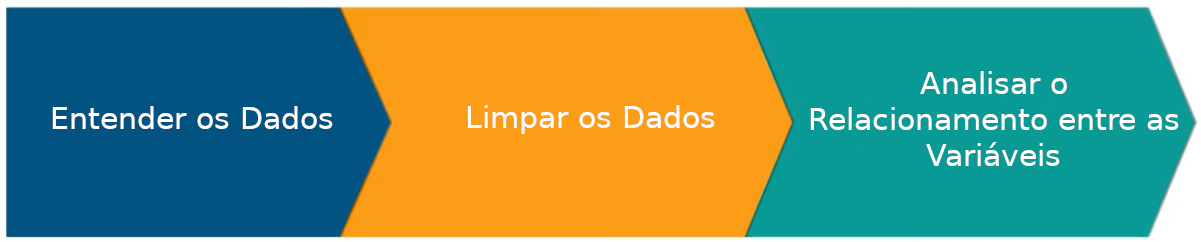
\includegraphics[width=0.6\textwidth]{cap03/EDA.png}
	\caption{Passos da EDA}
\end{figure}

A preparação dos dados para análise é inevitável, e a maneira como fazemos isso define a sua qualidade. Na prática o que faremos nesse capítulo é compreendermos o que temos a nossa disposição para trabalhar.

Normalmente os dados se dividem nas variáveis \textbf{Preditoras} (Entradas) e \textbf{Alvo} (saída). Uma vez que as localizamos devemos identificar o tipo de dados e a categoria das variáveis.

\section{Passo 1 - Entender os Dados}\index{EDA}
Nesta fase precisamos compreender o que temos a nossa disposição. Começamos o processo com a importação das bibliotecas:
\begin{lstlisting}
import pandas as pd
import matplotlib.pyplot as plt
import seaborn as sns
%matplotlib inline
\end{lstlisting}

Vamos trabalhar com três bibliotecas básicas, que como já mencionamos devemos conhecê-las a fundo: \textbf{Pandas} para análise dos dados, \textbf{MatPlotLib} e \textbf{SeaBorn} para mostrar os gráficos.

Agora precisamos dos dados, para isso usaremos o arquivo \textit{StudentsPerformance.csv}:
\begin{lstlisting}
df = pd.read_csv('StudentsPerformance.csv')
\end{lstlisting}

Nessa fase compreendemos melhor o que temos na nossa mão, \textbf{Pandas} é ideal para essa tarefa. Seu funcionamento é como um "Editor de Planilha", dessa forma que devemos encarar essa biblioteca, sua diferença básica é a nomenclatura de como o \textit{DataFrame} (e não Planilha) é visualizado:
\begin{figure}[H]
	\centering
	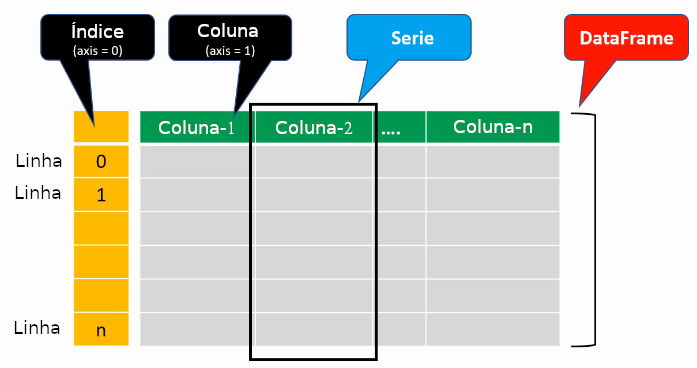
\includegraphics[width=0.7\textwidth]{cap03/PandasData.png}
	\caption{Visão Pandas}
\end{figure}

Uma coluna aqui é vista como uma \textit{Serie} e o \textit{index} é o que mantêm a "cola" das colunas. Dois comandos são básicos para visualizarmos o DataFrame:
\begin{lstlisting}
df.head()
\end{lstlisting}

Mostra as primeiras linhas, como parâmetro podemos passar a quantidade. E:
\begin{lstlisting}
df.tail()
\end{lstlisting}

Mostra as últimas linhas e também como parâmetro podemos passar a quantidade. O que temos até o momento? Sabemos é uma base sobre estudantes e as linhas são: gênero, etnicidade, nível de escolaridade dos pais, forma de alimentação, realizou um teste de preparação do curso, nota de matemática, nota de leitura e nota de escrita.

Então só com esses dois comandos já podemos saber sobre qual assunto iremos tratar: estudantes que realizaram provas e em quais condições. Quantos registros temos a nossa disposição? Ou quais são os nomes das colunas?
\begin{lstlisting}
print("Tamanho: ", df.shape)
print("Nome das Colunas: ", df.columns)
\end{lstlisting}

Estas variáveis respondem aos questionamentos. De forma mais completa podemos usar:
\begin{lstlisting}
df.info()
\end{lstlisting}

Que nos mostra inclusive qual o tipo de cada coluna e se esta contém ou não elementos nulos. Temos 3 colunas que são do tipo inteiro (int64), podemos analisá-las com o comando:
\begin{lstlisting}
df.describe()
\end{lstlisting}

Nos fornece as informações estatísticas básicas como média, desvio padrão, menor valor, máximo, 1º quartil (25\%), 2º quartil ou mediana (50\%), 3º quartil (75\%) e o maior valor. Ou seja, as informações para a montagem de um \textbf{BoxPlot}. Vamos montá-lo para melhor visualizar os dados:
\begin{lstlisting}
fig, axes = plt.subplots(1, 3, figsize=(10,4))
axes[0].boxplot(df['math score'])
axes[0].set_title("Matemática")
axes[1].boxplot(df['reading score'])
axes[1].set_title("Leitura")
axes[2].boxplot(df['writing score'])
axes[2].set_title("Escrita")
plt.show()
\end{lstlisting}

E obtemos como resultado:
\begin{figure}[H]
	\centering
	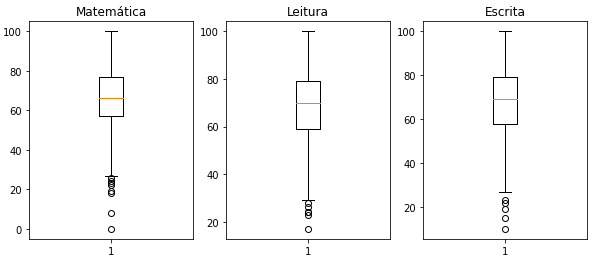
\includegraphics[width=0.55\textwidth]{cap03/BoxPlot.png}
	\caption{BoxPlot das Notas}
\end{figure}

\textbf{Boxplot}\footnote{Diagrama de Caixa se prefere, foi atribuída ao matemático \textbf{John W. Tukey} (1915 –2000), curiosamente algumas literaturas chamam de "\textit{Tukey BoxPlot}", mas se realizar uma pesquisa ninguém sabe ao certo quem criou realmente esse diagrama.} é um gráfico que avalia a distribuição dos dados. É formado exatamente com os dados que mostramos na função \textit{describe()}. Porém suas hastes (inferiores e superiores) se estendem do quartil inferior (ou superior) até o menor valor não inferior (ou superior) ao limite. São calculados da seguinte forma: \vspace{-1em}
\begin{itemize}
	\item Limite inferior: $Q_1 - 1,5 \times (Q_3 - Q_1)$.
	\item Limite superior: $Q_3 + 1,5 \times (Q_3 - Q_1)$.
\end{itemize}

Resumidamente é formado da seguinte maneira:
\begin{figure}[H]
	\centering
	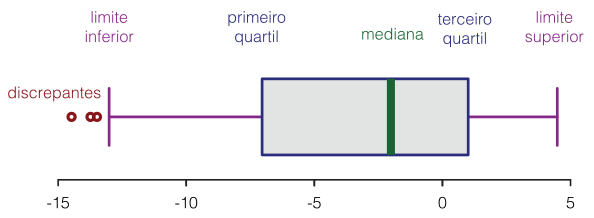
\includegraphics[width=0.6\textwidth]{cap03/estrutBoxplot.png}
	\caption{Estrutura do BoxPlot}
\end{figure}

Esses pontos "discrepantes" podem ocorrer acima ou abaixo dos limites, são chamados de \textit{Outliers}. Não é necessariamente um erro, podemos classificá-lo como uma anomalia curiosa e que merece nossa atenção.

\subsection{Localizar os Outliers}\index{EDA}
Para achar esses \textit{Outliers} isolamos as três colunas numéricas:
\begin{lstlisting}
X = df.iloc[:, 5:8].values
\end{lstlisting}

E criamos um novo DataFrame somente com essas com a modificação do seu nome por um número:
\begin{lstlisting}
pd.options.display.float\_format = '{:.1f}'.format
xDF = pd.DataFrame(X)
\end{lstlisting}

Para quê isso serve? A função \textit{describe()} cria um DataFrame, podemos percorrê-lo, porém fica muito mais simples se cada coluna for um numeral, pois assim podemos usar um comando \textit{for} para isso:
\begin{lstlisting}
z = xDF.describe()
for t in z:
  iqr = z[t][6] - z[t][4]
  extMenor = z[t][4] - (iqr * 1.5)
  extMaior = z[t][6] + (iqr * 1.5)
  print('Na Col. \%d devem estar abaixo de \%.2f e acima de \%.2f' \% (t, extMenor, extMaior))
\end{lstlisting}

E obtemos o seguinte resultado: \\
\codigo{Na Col. 0 devem estar abaixo de 27.00 e acima de 107.00 \\
Na Col. 1 devem estar abaixo de 29.00 e acima de 109.00 \\
Na Col. 2 devem estar abaixo de 25.88 e acima de 110.88}

Pelo BoxPlot todos os valores estão abaixos, então para localizá-los:
\begin{lstlisting}
matOutliers = (X[:,0] < 27)
df[matOutliers]
\end{lstlisting}

Localizamos todas linhas que a nota de matemática (coluna 0) seja abaixo de 27 e mostramos esses registros. Podemos proceder de modo semelhante para as notas de leitura (coluna 1) e escrita (coluna 2) e assim desvendar quem são os \textit{Outliers}.

Podemos também analisar graficamente, e visualizar a Distribuição Normal de cada variável, por exemplo para a nota de Escrita:
\begin{lstlisting}
sns.kdeplot(df['writing score'], shade=True)
plt.show()
\end{lstlisting}

Obtemos como resultado:
\begin{figure}[H]
	\centering
	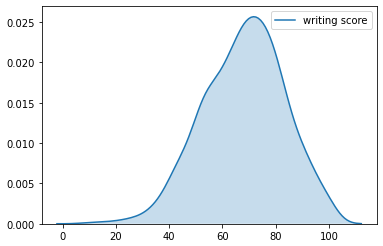
\includegraphics[width=0.5\textwidth]{cap03/NotaEscrita.png}
	\caption{Distribuição dos Dados para Nota de Escrita}
\end{figure}

E assim verificamos como cada atributo numérico se comporta.

\subsection{Colunas Categóricas}\index{EDA}
Sabemos que as primeiras cinco colunas do nosso Dataframe são categóricas, porém conforme a função info() o tipo delas estás \textit{object}. É interessante mudarmos para o tipo caractere para evitarmos quaisquer problemas futuros.
\begin{lstlisting}
df['gender'] = df['gender'].astype(pd.StringDtype())
df['race/ethnicity'] = df['race/ethnicity'].astype(pd.StringDtype())
df['parental level of education'] = df['parental level of education'].astype(pd.StringDtype())
df['lunch'] = df['lunch'].astype(pd.StringDtype())
df['test preparation course'] = df['test preparation course'].astype(pd.StringDtype())
\end{lstlisting}

E ao aplicarmos uma nova chamada a função \textit{info()} vemos que os tipos agora estão corretos. Quantos tipos únicos existem em cada uma dessas colunas?
\begin{lstlisting}
df.nunique()
\end{lstlisting}

Mostra a quantidade de valores não repetidos em cada coluna (inclusive as numéricas). E agora sabemos que temos: 2 gêneros, 5 etnicidades, 6 níveis de escolaridade dos pais, 2 formas de alimentação e 2 tipos para teste de preparação do curso. Mas quem são eles?
\begin{lstlisting}
print("Gênero: ", df['gender'].unique())
print("Etinicidade: ", df['race/ethnicity'].unique())
print("Escolaridade dos Pais: ", df['parental level of education'].unique())
print("Refeição: ", df['lunch'].unique())
print("Realizou Preparatório: ", df['test preparation course'].unique())
\end{lstlisting}

\section{Passo 2 - Limpar os Dados}\index{EDA}
A limpeza dos dados trata de muitos problemas como informação repetida, valores faltantes (que podem ser descobertos por associação) e inconsistentes. Para esse último tipo o pior caso são os nulos. (In)felizmente essa base está horrível para essa fase e assim pegamos um outro arquivo \textbf{titanic.csv}: 
\begin{lstlisting}
df = pd.read_csv('titanic.csv')
df.head()
\end{lstlisting}

Repetimos todo o processo da fase anterior para descobrirmos de que se tratam os dados e descobrimos que são os dados dos passageiros (sobreviventes ou não - coluna \textit{Survived} - sendo esta a coluna alvo da base) do famoso \textbf{RMS Titanic} que foi pensado para ser o navio mais luxuoso e seguro de sua época e supostamente "inafundável". Como sabemos em sua viagem inaugural de \textit{Southampton} para \textit{Nova Iorque} afundou no dia 14 de abril de 1912 com mais de 1.500 pessoas a bordo. Porém esta base contém apenas 891 registros.

Ao aplicarmos a função info() percebemos que as colunas \textit{Age} (idade), \textit{Cabin} (número da cabine) e \textit{Embarked} (local de Embarque) possuem dados faltantes. Que dados são esses?
\begin{lstlisting}
print(df.isnull().sum())
\end{lstlisting}

Sabemos que faltam: 177 em \textbf{Age}, 687 em \textbf{Cabin} e 2 em \textit{Embarked}. Também podemos mostrar exclusivamente os que faltam, isso é útil para quando temos muitas colunas no modelo:
\begin{lstlisting}
null_value_stats = df.isnull().sum(axis=0)
null_value_stats[null_value_stats != 0]
\end{lstlisting}

Ou ainda criar uma função que nos retorna um Dataframe com a informação mais completa o possível (inclusive com o percentual):
\begin{lstlisting}
def mostrarNulos(data):
  null_sum = data.isnull().sum()
  total = null_sum.sort_values(ascending=False)
  percent = (((null_sum / len(data.index))*100).round(2)).sort_values(ascending=False)
  df_NULL = pd.concat([total, percent], axis=1, keys=['Tot.Nulo', 'Perc.Nulo'])
  df_NULL = df_NULL[(df_NULL.T != 0).any()]
  return df_NULL
\end{lstlisting}

E ao chamá-la:
\begin{lstlisting}
df_Age = mostrarNulos(df)
df_Age.head()
\end{lstlisting}

Obtemos como resultado:
\begin{figure}[H]
	\centering
	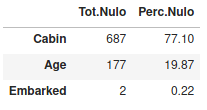
\includegraphics[width=0.3\textwidth]{cap03/TitanicNulosPerc.png}
	\caption{Nulos e Percetual da Base Titanic}
\end{figure}

Lidar com esses tipos de nulos é complicado pois não temos como consultar e o máximo que podemos fazer é podá-los da nossa base ou atribuir um valor genérico que não afete nosso resultado (como o caso de \textit{Embarked}). Porém \textbf{Número da Cabine} é um dado relevante? Essa é a principal pergunta que nos devemos fazer, por exemplo existe algum modelo preditivo que possa nos dizer que se estivéssemos em determinada cabine no navio sobreviveríamos ou não? Entretanto \textbf{Idade} é um dado relevante (lembra da frase: mulheres e crianças primeiro), então essa é uma característica que pode ser essencial.

Criar uma função com um gráfico para mostrar, por idade, como estão os dados:
\begin{lstlisting}
def executarGrafico():
  try:
    sns.distplot([df['Age']])
    plt.show()
  except ValueError as err:
    print(err) 
\end{lstlisting}

Agora a cada vez que chamarmos essa função obtemos como resultado:
\begin{figure}[H]
	\centering
	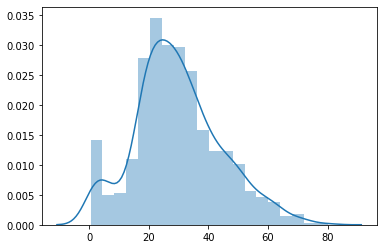
\includegraphics[width=0.45\textwidth]{cap03/TitanicIdade1.png}
	\caption{Gráfico de Idade do Titanic}
\end{figure}

\begin{note}[Imputação ou retirada de valores] 
	Como tratamos de adicionar ou retirar dados na base a cada vez devemos ler novamente os dados do arquivo CSV.
\end{note}

Porém em algumas versões da SeaBorn este pode apresentar erro devido a presença dos nulos, é ideal que os retiremos do \textit{DataFrame} para evitarmos problemas. Em muitas biografias encontramos algo do tipo: "atribuir um valor (preferencialmente \textit{outlier}) para estes tipos". Tentaremos essa técnica com os seguintes comandos:
\begin{lstlisting}
df['Age'].fillna(-25, inplace=True)
executarGrafico()
\end{lstlisting}

Obtemos como resultado:
\begin{figure}[H]
	\centering
	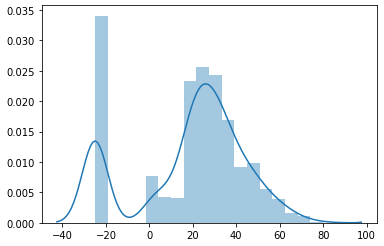
\includegraphics[width=0.45\textwidth]{cap03/TitanicIdade2.png}
	\caption{Gráfico de Idade do Titanic com Outliers}
\end{figure}

Nosso gráfico de idade agora ganhou uma coluna, que sabemos com valores não existentes, também podemos atribuir qualquer outro valor como por exemplo a média:
\begin{lstlisting}
df['Age'] = df['Age'].fillna(df['Age'].mean())
executarGrafico()
\end{lstlisting}

Ou a mediana (função median()) que resultaria em um gráfico completamente esquisito. Sendo assim vamos cortar esses valores:
\begin{lstlisting}
df = df.dropna(axis=0)
executarGrafico()
\end{lstlisting}

E teremos a seguinte situação:
\begin{figure}[H]
	\centering
	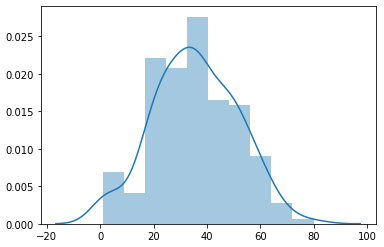
\includegraphics[width=0.45\textwidth]{cap03/TitanicIdade3.png}
	\caption{Gráfico de Idade do Titanic sem nulos}
\end{figure}

O que aconteceu? O comando executado eliminou todas as linhas que possuiam valores nulos, a coluna \textit{Cabin} interferiu e nos resultou, conforme pode ser mostrado com a função \textit{info()} em somente 183 registros no total. Ou seja, o corte que devemos aplicar deve ser cirúrgico e somente na coluna idade.
\begin{lstlisting}
df['Age'] = df['Age'].dropna(axis=0)
executarGrafico()
\end{lstlisting}

O que nos resulta no mesmo gráfico mostrado no início desta e 891 registros. E como citamos podemos arrancar a coluna \textit{Cabin} para que esta não interfira mais:
\begin{lstlisting}
df = df.drop(['Cabin'], axis=1)
\end{lstlisting}

\begin{note}[Ferramenta para Limpeza dos Dados] 
	Conhece o \textbf{OpenRefine?} é uma ferramenta gratuita dedicada a limpeza e tratamento dos dados baixe um paper sobre o OpenRefine gratuitamente na minha página no Academia.edu (\url{https://iesbpreve.academia.edu/FernandoAnselmo}).
\end{note}

\section{Passo 3 - Relacionamento entre as Variáveis}\index{EDA}
Vamos retomar nossa base de \textbf{Estudantes} e verificarmos como as variáveis se relacionam:
\begin{lstlisting}
df = pd.read_csv('StudentsPerformance.csv')
df.corr()
\end{lstlisting}

E temos o relacionamento o grau de como as variáveis que se relacionam, esse número varia de -1 a 1, sendo o negativo um relacionamento nulo. Porém é muito mais fácil de vermos esse resultado com um Mapa de Calor:
\begin{lstlisting}
rel = df.corr()
sns.heatmap(rel, xticklabels=rel.columns, yticklabels=rel.columns, annot=True)
plt.show()
\end{lstlisting}

Obtemos como resultado:
\begin{figure}[H]
	\centering
	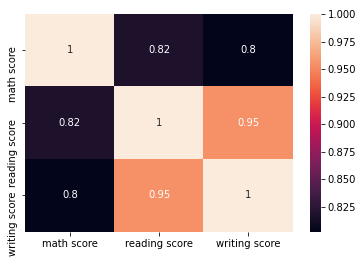
\includegraphics[width=0.5\textwidth]{cap03/MapaDeCalor.png}
	\caption{Mapa de Calor dos Relacionamentos}
\end{figure}

Vemos que as notas de Escrita e Leitura possuem um forte grau de relacionamento, como se uma fosse a responsável pela outra. Já a de matemática interfere mais na nota de leitura.

Curiosamente se aplicarmos isso na base do \textbf{Titanic} veremos que as colunas mais importantes para \textit{Fare} (sobreviveu) que é nossa variável alvo são: \textit{Fare} que é o valor pago pela passagem e \textit{Parch} que se refere a quantidade de pais. Ou seja, os mais ricos e se a criança tinha ou não os pais a bordo. 

Outra maneira de visualizarmos, também de forma gráfica, é através de uma dispersão de valores:
\begin{lstlisting}
sns.pairplot(df)
plt.show()
\end{lstlisting}

Obtemos como resultado:
\begin{figure}[H]
	\centering
	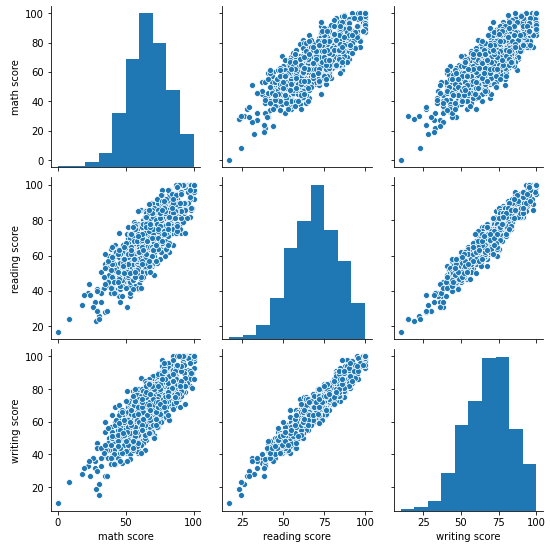
\includegraphics[width=0.7\textwidth]{cap03/dispersao.png}
	\caption{Dispersão Associada}
\end{figure}

Quanto mais juntos aparecem os pontos mais relacionadas estão. Podemos isolar as notas de Escrita e Leitura em um único gráfico, por exemplo:
\begin{lstlisting}
sns.regplot(x='writing score', y='reading score', data=df)
plt.show()
\end{lstlisting}

Esta função executa um ajuste e plotagem simples com base no modelo de Regressão Linear. E obtemos como resultado:
\begin{figure}[H]
	\centering
	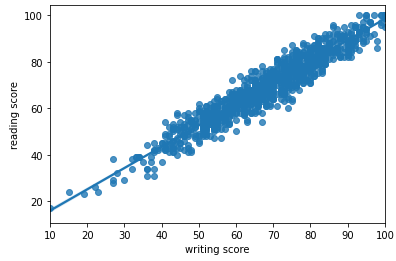
\includegraphics[width=0.55\textwidth]{cap03/NotasRegress.png}
	\caption{Notas de Leitura e Escrita}
\end{figure}

Porém o mais interessante é colorir os pontos de forma diferente com base em uma variável categórica que achamos que pode ser uma causa (para uma nota alta ou baixa), por exemplo o quanto a alimentação interferiu na nota:
\begin{lstlisting}
sns.lmplot(x='writing score', y='reading score', hue='lunch', data=df)
plt.show()
\end{lstlisting}

A função \textit{lmplot()} combina \textit{regplot()} com a classe \textbf{FacetGrid}. Esta classe auxilia visualizar a distribuição de uma variável, bem como o relacionamento entre várias variáveis separadamente dentro de subconjuntos do seu conjunto de dados. E obtemos como resultado:
\begin{figure}[H]
	\centering
	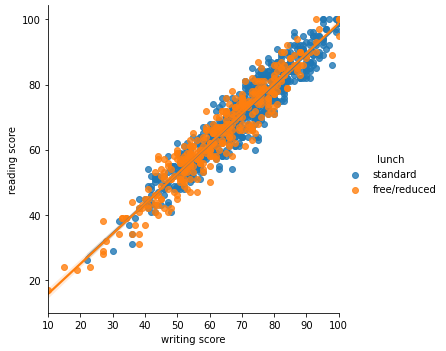
\includegraphics[width=0.5\textwidth]{cap03/NotasLmplot.png}
	\caption{Nota associada a Alimentação - RegPlot}
\end{figure}

Uma melhor forma de visualizar é usar a função \textit{relplot()} que fornece acesso a várias funções diferentes no nível de eixos que mostram o relacionamento entre as duas variáveis com mapeamentos semânticos de subconjuntos:
\begin{lstlisting}
sns.relplot(x='writing score', y='reading score', hue='lunch', data=df)
plt.show()
\end{lstlisting}

Obtemos como resultado:
\begin{figure}[H]
	\centering
	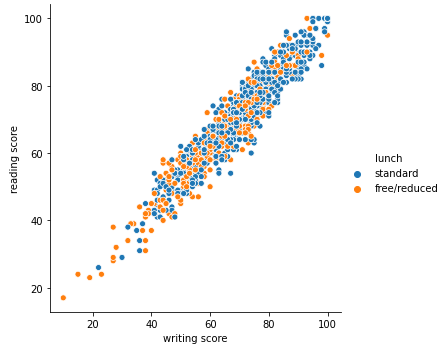
\includegraphics[width=0.55\textwidth]{cap03/NotasAlimentacao.png}
	\caption{Nota associada a Alimentação - RelPlot}
\end{figure}

Ou seja, podemos responder várias perguntas apenas com a verificação do relacionamento entre os atributos, tente realizar o mesmo teste com as outras variáveis categóricas e descobrir como essas se comportam na nota, se existe ou não interferência. 

\section{Conclusão}\index{EDA}
Mantemos em mente que EDA e um aspecto central da \textit{Data Science}, que às vezes é esquecido. O primeiro passo de qualquer ação que tomemos é conhecer os dados: entendê-los, familiarizar-se com eles. Quais são as respostas que estamos tentando obter dos dados? Quais são as variáveis e o que elas significam? Como é a aparência de uma perspectiva estatística? Os dados estão formatados corretamente? Tem valores ausentes? duplicados? E quanto aos \textit{outliers}? Conhecemos eles? Ou seja, devemos responder a esses questionamentos.

É necessário muito trabalho de preparação, porque os dados no mundo real raramente são limpos e homogêneos. Costumamos dizer que 80\% do tempo valioso de um cientista de dados é gasto simplesmente com a localização, limpeza e organização dados. Os 20\% restantes são para realmente realizar as análises.

Agora estamos prontos para começarmos a explorar diversas bases de dados com a utilização dos modelos.